\section{Akcelerometr trzyosiowy}
W latach 90 akcelerometry instalowano jedynie w roli mechanizmów służących do
uruchamiania poduszek powietrznych w samochodzie w przypadku wystąpienia
zderzenia. W chwili obecnej akcelerometry wykonane w technologii
MEMS można znaleźć w większości urządzeń codziennego użytku tj.
telefony komórkowe, konsole do gier, komputery przenośne czy cyfrowe aparaty
fotograficzne. Powodem tak spektakularnego wzrostu popularności było pełne
rozwinięcie się technologii MEMS. W dobie miniaturyzacji fakt, iż w miejsce do
niedawna używanych urządzeń można wstawić pojedynczy układ
scalony jest jednym z podstawowych powodów dla których, między innymi,
akcelerometry cieszą się tak szerokim spektrum zastosowań. Jednakże, ceną tak
daleko idącej miniaturyzacji jest spadek duży dokładności pomiarowej w
porównaniu do akcelerometrów opartych o tensometry. Jak się jednak okazuje, do
codziennego użytku precyzja oferowana przez tego typu czujniki jest w zupełności wystarczająca.

Bardzo dobrym przykładem zastosowania akcelerometru jest dostępna w większości
aparatów cyfrowych funkcja optycznej stabilizacji obrazu (Optical Image
Stabilization). Funkcja ta polega na redukcji zniekształceń  spowodowanych
drżeniem rąk fotografa w~trakcie akwizycji obrazu. Problem jest tym poważniejszy
iż nieustanna miniaturyzacja urządzeń dodatkowo wzmacnia mimowolne\footnote{Ręka
przeciętnego człowieka drży mimowolnie z częstotliwością od 10 do 20 Hz} drżenie
rąk użytkownika. Dlatego też większość aparatów wyposażonych jest czujniki które
mierzą wspomniane drgania, a następnie uzyskane informacje przekazują do modułu
sterującego położeniem soczewek i przetwornika obrazu. Następnie moduł ten
dostosowuje parametry pracy aparatu tak aby zminimalizować wpływ nieporządanych przeunięć
na efekt końcowy pracy jakim jest zdjęcie.

Innym popularnym przykładem zastosowania akcelerometrów są pedometry, potocznie 
nazywane krokomierzami. Dzięki zastosowanej technologii czujniki w krokomierzach
mogą dokonywać równocześnie pomiaru względem trzech osi. Co więcej tego typu
urządzenia umożliwiają dokonywanie pomiarów niemal całkowicie niezależne od
swojej orientacji, a ich niewielkie rozmiary pozwalają na ich integrację z 
dowolnymi urządzeniami mobilnymi. Akcelerometry wykonane w technologi MEMS
najlepiej sprawdzają się  podczas pomiaru przyspieszenia statycznego
pozwalającego jednoznacznie wyznaczyć kąt odchylenia urządzenia względem pionu. 
Można nimi dokonywać również pomiaru przyspieszenia dynamicznego pojawiającego 
się na skutek wibracji, uderzenia czy innego rodzaju ruchu. 

Niestety, pomimo swoich licznych zalet akcelerometry MEMS posiadają pewne
ograniczenia które mogą być bardzo istotne podczas projektowania bardziej
skomplikowanych systemów. Jedynym z podstawowych problemów jest brak możliwości
uzyskania jednoznacznej informacji na temat orientacji urządzenia zarówno w
pionie jak i poziomie. W~ramach przykładu spróbujmy przeanalizować wykorzystanie
akcelerometru do przełączania widoku na ekranie w zależności od jego orientacji. 
W~przypadku gdy oś X lub Y są równoległe z wektorem grawitacji na podstawie
informacji z akcelerometru można w~bardzo prosty sposób ustalić w~jakim
położeniu znajduje się aktualnie urządzenie.

\begin{figure}[ht!]
 \centering
 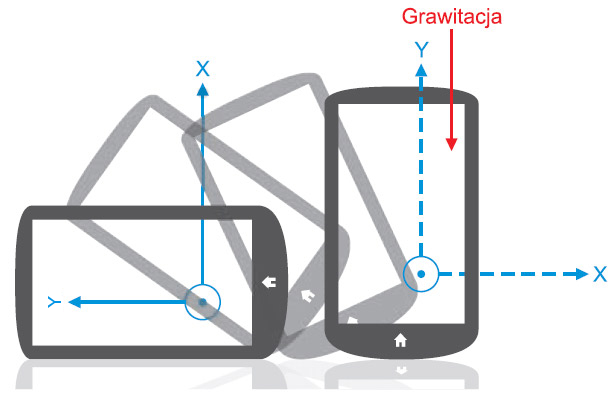
\includegraphics[height=75mm]{../images/ch04/acc_orientation.png}
 \caption{Pokrywanie się osi ekranu z kierunkiem wektora grawitacji pozwala na
 precyzyjne wyznaczenia orientacji urządzenia\cite{website:elektronikab2b-zyroskop}}
 \label{fig:AkcelerometrOrientation}
\end{figure}

Natomiast w przypadku gdy osie ekranu ustawią się prostopadle do wektora
grawitacji dane pozyskane z akcelerometru nie pozwalają na wyznaczenie
jednoznacznej pozycji w jakiej znalazło się urządzenie\cite{website:elektronikab2b-zyroskop}. Co więcej w
przypadku aplikacji w których akcelerometr jest źródłem informacji o odchyleniu od pionu
konieczne jest rozdzielenie zmian związanych wpływem grawitacji od szumów
związanych z przyspieszeniem dynamicznym. Tak pozyskane informacje będą
służyć jako punkt odniesienia pozwalającego na wyznaczenie kąta wychylenia.
Głównym problemem jest fakt, że sygnał taki można wyróżnić jedynie w chwili gdy
akcelerometr jest w stanie spoczynku, co w przypadku niektórych rodzajów
zastosowań może dawać nieoczekiwane rezultaty i zachwiać stabilność pracy całego
systemu. 

Jeżeli założymy, że zmiany odpowiadające przyspieszeniu dynamicznemu mają dużą
częstotliwość to możemy przy użyciu filtru dolnoprzepustowego usunąć zakłócenia
związane z drganiami wywołanymi przez użytkownika. Oczywistą implikacją
powyższego założenia jest założenie, że zmiana kąta nachylenia względem pionu są
wolne. W przeciwnym wypadku informacja o zmianie odchylenia zostaną usunięte
przez wspomniany filtr. Aby pominięcie wspomnianych ograniczeń stało się możliwe
konieczne jest zastosowanie dodatkowych czujników takich jak np. żyroskop które
dostarczą uzupełniających informacji pozwalających na stabilną implementację
funkcjonalności.

\subsection{Rodzaje akcelerometrów}
Istnieje wiele różnych rodzajów akcelerometrów. Akcelerometry mechaniczne
przypominają po części zachowanie pasażera w samochodzie który gwałtowanie
przyspiesza i zwalnia. Posiadają one element masy przyczepiony do elementu
sprężynowego umieszczonego w całości w zewnętrznej obudowie. Kiedy taki
akcelerometr zacznie przyspieszać obudowa zewnętrzna przemieści się podczas gdy
punkt masy wychyli się w kierunku przeciwnym do przyspieszenia co spowoduje
rozciągnięcie się sprężyny wprost proporcjonalne do siły która spowodowała
przyspieszenie. Mierząc więc odległość na jaką nastąpiło wychylenie jesteśmy w
stanie wyznaczyć wartość działającej siły, a co za tym idzie również wartość
przyspieszenia. Opisana powyżej zasada pomiaru leży u podstaw działania
sesjsmografów które za pomocą masy dołączonej do elementu piśmiennego rejestrują
siły występujące w chwili trzęsienia ziemi.

Alternatywnym podejściem jest wykorzystanie sygnałów elektrycznych i
magnetycznych do pomiaru przyspieszenia. Wśród tego rodzaju akcelerometrów
możemy wyróżnić następujące trzy typy: akcelerometr piezorezystywny,
akcelerometr pojemnościowy oraz akcelerometr piezoelektryczny. Istnieją również
akcelerometry które dokonują pomiaru przyspieszenia w oparciu o efekt Halla. 

\begin{figure}[ht!]
 \centering
 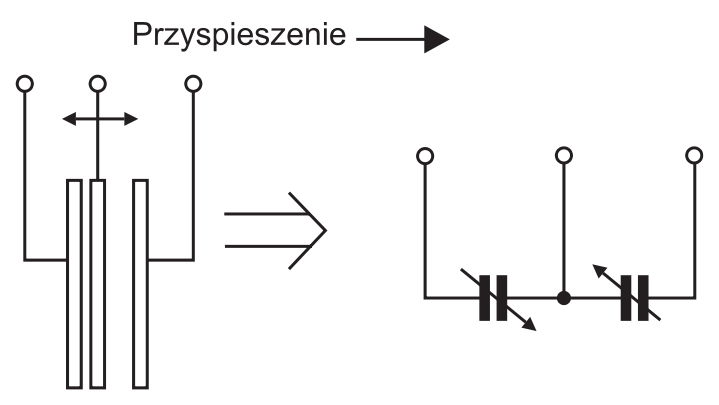
\includegraphics[height=62mm]{../images/ch04/acc_intro.png}
 \caption{Schemat ideowy akcelerometu pojemnościowego dokonującego pomiaru
 wzdłuż jednej osi\cite{ElektronikaPraktyczna22010}}
 \label{fig:AkcelerometrIdeowyScheamt}
\end{figure}

Przyspieszomierze piezorezystywne mają punkt masy dołączony do potencjometru
który zwiększa i zmniejsza przepływ prądu w zależności od siły jaka oddziałuje
na czujnik. Bardzo podobną zasadę działania wykazują akcelerometry pojemnościowe
te jednak wykorzystują efekt zmiany pojemności kondensatorów zastosowanych w
miejscu w którym poprzednio użyty został potencjometr. Ostatnim rodzajem
akcelerometrów są urządzeniami bazujące na piezoelektrycznych kryształach takich
jak na przykład kwarc. W urządzeniach tych punkt masy, pod wpływem
przyspieszenia, naciska na kryształ co powoduje, powstawanie napięcia które
jest wykorzystywane do wykonywania pomiaru. Cechą charakterystyczną tego rodzaju
czujników jest brak wskazań wartości przyspieszenia statycznego.\cite{website:elektronikab2b-platforma-bezzalogowa}

\subsection{Algorytm rozpoznawania kroków}
Do poprawnego działania algorytmu zaprezentowanego w ramach noty
aplikacyjnej\cite{Pedometer-haam326b} wymagane jest wykorzystanie akcelerometru
trójosiowego. Jak już wspomniano wcześniej, dzięki zastosowaniu urządzenia tego
typu jesteśmy w stanie wyeliminować problemy wynikające z konieczności 
uwzględnienia aktualnego wychylenia akcelerometru względem wektora grawitacji. 
W przypadku gdyby możliwe byłoby korzystanie tylko z pojedynczych osi poprawne
działanie algorytmu byłoby zapewnione jedynie w ściśle określonej pozycji co
jest znaczącym utrudnieniem biorąc pod uwagę niehomogeniczny charakter ruchów
wykonywanych podczas chodzenia. Aby wyeliminować wspomniany problem do
ostatecznego rozwiązania brana jest jedynie wartość stanowiąca złożenie wartości
przyspieszenia dla poszczególnych osi. Do wyznaczenia bezwzględnego
przyspieszenia na podstawie danych z osi X, Y, Z użyte zostało równanie
\ref{eq:AccCompositEq}.
\begin{equation}
a_{xyz} = \sqrt{{a_x}^2 + {a_y}^2 + {a_z}^2}
\label{eq:AccCompositEq}
\end{equation}
Zaimplementowany w ramach pracy magisterskiej algorytm wykrywania i zliczania
kroków bazuje na założeniu iż sumaryczna wartość przyspieszenia wykrywanego
przez akcelerometr w trakcie chodzenia oscyluje wokół wartości 1G\footnote{1G
- Jednokrotność przyspieszenia ziemskiego wynoszącego w przybliżeniu 9.81
$\frac{m}{s^2}$}. Podstawową zasadą działania algorytmu jest więc wykrywanie
cykli w jakich następuje kolejno spadek wartości odczytywanego przyspieszenia, a
następnie jego wzrost ponad wartość spoczynkową. Do poprawnego działania
algorytmu konieczne jest dobranie nie tylko odpowidniej stałej czasowej w której
wykryty cykl będzie zliczany jako krok, ale również ustalenie progów
przyspieszenia poniżej i powyżej wartości spoczynkowej które będą traktowane
jako odpowiednio początek i koniec cyklu.

\subsection{Implementacja algorytmu}
Do praktycznej implementacji algorytmu wykrywania kroków wykorzystany został
moduł akcelerometru trójosiowego firmy Freescale Semiconductor. Czujnik 
MMA7260\cite{MMA7260DataSheet} został zainstalowany w robocie jako element
modułu MOBOT-GM3A. Moduł akcelerometru jest to jedyny moduł w całości
dostarczony przez zewnętrznego dostawce, a wybór takiej strategii podyktowany
był jedynie względami ekonomicznymi i dostępnością tego typu urządzeń na polskim
rynku elektronicznym. Na ilustracji zamiszczone zostało zdjęcie gotowego układu
wraz z zaznaczonymi wyprowadzeniami.

\begin{figure}[ht!]
 \centering
 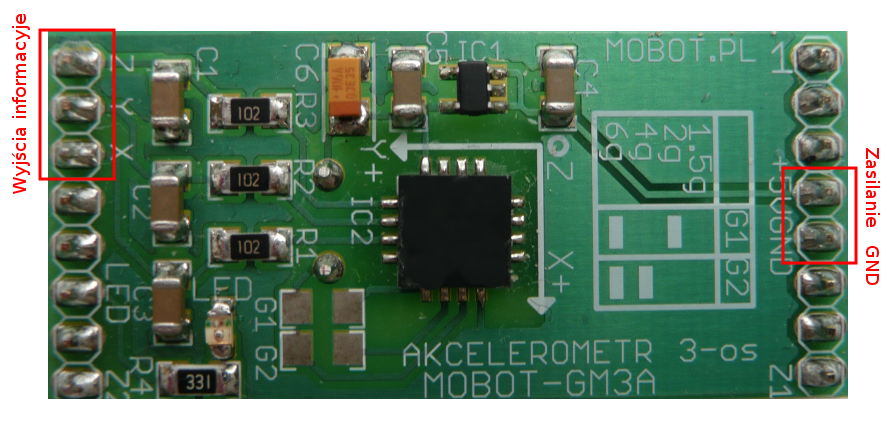
\includegraphics[height=76mm]{../images/ch04/gm3a_view.png}
 \caption{Moduł akcelerometru trójosiowego z czujnikiem przyspieszenia MMA7260}
 \label{fig:AccView}
\end{figure}

Wykorzystany czójnik przyspieszenia oferuje cztery zakresy czułości których
zmiana odbywa się poprzez konifguraję odpowiednich zworek w module MOBOT - GM3A.
W~ramach implementacji wybrany został zakres czułości od $-1.5g$ do $1.5g$ gdyż
udziela on najdokładniejszej informacji na temat przyspieszenia w przedziale w
jakim mieszczą się przyspieszenia związane z chodzeniem. W wybranym trybie
czułości akcelerometr wykazuje czułość rzędu 800mV/g, co przy wartości
przyspieszenia równej zero daje środek przedziału czułości na poziomie 1.65V.
Ze względu na analogową charakterystykę sygnału wyjściowego z modułu
akcelerometru konieczne jest wykorzystanie konwertera analogowo-cyfrowego w
celu odczytania danych pomiarowych otrzymywanych na wyjściach urządzenia.
Szczegółowy opis działania wbudowanego w robota ADC można znaleźć w rozdziale
poświęconym dalmierzom IR. 

\begin{figure}[ht!]
 \centering
 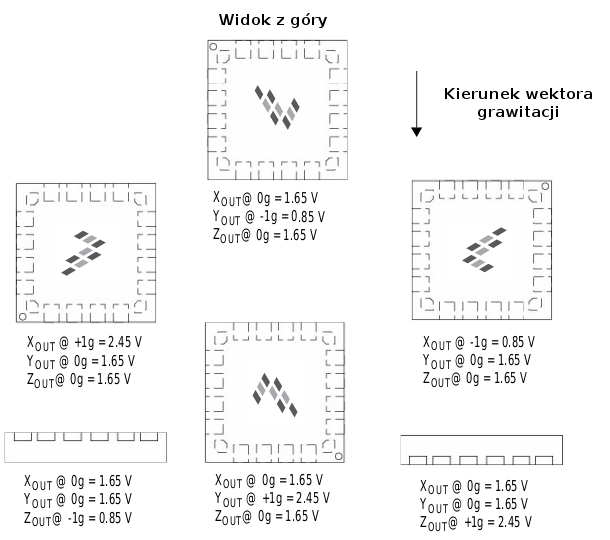
\includegraphics[height=75mm]{../images/ch04/mma7260_datasheet.png}
 \caption{Wartości przyspiesznia statycznego dla układu MMA7260 dostarczone w
 ramach specyfikacji technicznej urządzenia\cite{MMA7260DataSheet}}
 \label{fig:MMADataSheetStaticAcc}
\end{figure}

Przed rozpoczęciem praktycznej implementacji alogrytmu wykrywania kroków
konieczne okazało się przeprowadzenie kalibracji modułu, gdyż już wstępne testy
czujnika zwróciły spore różnice pomiędzy wartościami podanymi w nocie
katalogowej, a stanem zmierzonym na wyjściach akcelerometru. Zgodnie z rysunkiem
znalezionym w dokumentacji udostępnionej przez producenta czułość oraz zakres
napięć na poszczególnych osiach powinien być w stałych, jednakowych
przedziałach. Niestety jak się okazało poszczególne osie miały bardzo znaczące
różnice w zakresie swojej czułości co mogłoby bardzo niekorzystnie wpłynąć na
stabilność działania zaproponowanego algorytmu zliczania kroków. 

\begin{figure}[ht!]
 \centering
 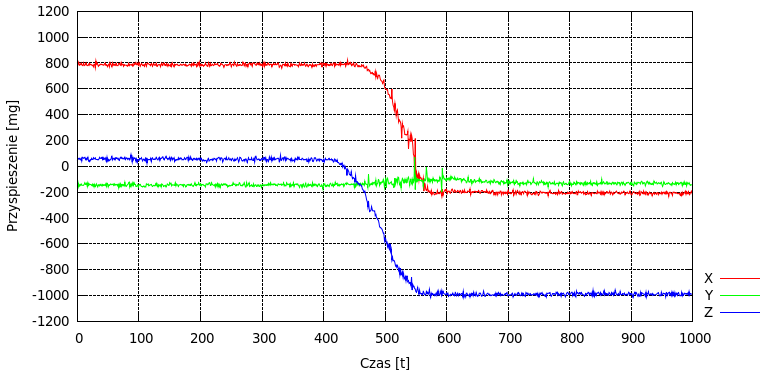
\includegraphics[height=80mm]{../images/ch04/raw_acc_data.png}
 \caption{Wartości przyspiezenia odczytywane na wyjściach akcelerometru przed
 przeprowadzeniem kalibracji}
 \label{fig:MMADataRaw}
\end{figure}

Wspomniany proces kalibracji polegał na ustawieniu czujnika na płaskiej,
poziomej powierzchni oraz odczytaniu wartości przyspieszenia statycznego dla
każdej z osi z osobna. Procedurę taką powtarzano wielokrotnie zmieniając
orientację modułu względem wektora grawitacji. Po zebraniu wszystkich danych
pomiarowych dla każdej osi z osobna została wyznaczona rzeczywista czułość, a
następnie w module odpowiedzialnym za akwicyzję danych o przyspieszeniu zostały
zaprogramowane funkcje korygujące otrzymane dane wejściowe o wartości wyliczone
podczas kalibracji urządzenia. Na poniższych wykresach znajdują się informacje o
stanie wyjść przed i po przeprowadzeniu kalibracji. 
  
\begin{figure}[ht!]
 \centering
 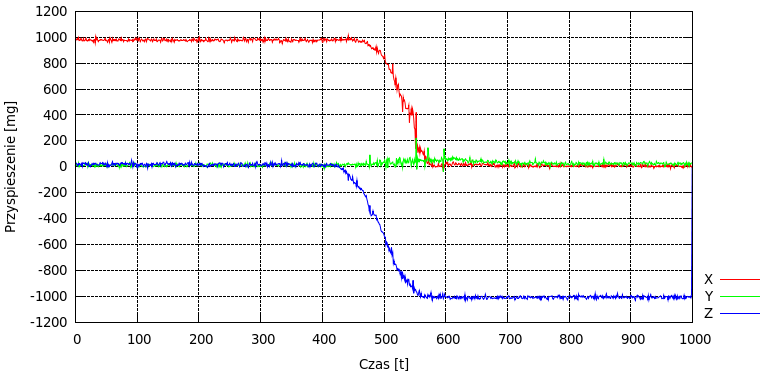
\includegraphics[height=80mm]{../images/ch04/calib_acc_data.png}
 \caption{Wartości odczytywane na wyjściach akcelerometru po przeprowadzeniu kalibracji}
 \label{fig:MMADataCalib}
\end{figure}